% Options for packages loaded elsewhere
\PassOptionsToPackage{unicode}{hyperref}
\PassOptionsToPackage{hyphens}{url}
\PassOptionsToPackage{dvipsnames,svgnames*,x11names*}{xcolor}
%
\documentclass[
  11pt,
]{book}
\usepackage{lmodern}
\usepackage{amssymb,amsmath}
\usepackage{ifxetex,ifluatex}
\ifnum 0\ifxetex 1\fi\ifluatex 1\fi=0 % if pdftex
  \usepackage[T1]{fontenc}
  \usepackage[utf8]{inputenc}
  \usepackage{textcomp} % provide euro and other symbols
\else % if luatex or xetex
  \usepackage{unicode-math}
  \defaultfontfeatures{Scale=MatchLowercase}
  \defaultfontfeatures[\rmfamily]{Ligatures=TeX,Scale=1}
\fi
% Use upquote if available, for straight quotes in verbatim environments
\IfFileExists{upquote.sty}{\usepackage{upquote}}{}
\IfFileExists{microtype.sty}{% use microtype if available
  \usepackage[]{microtype}
  \UseMicrotypeSet[protrusion]{basicmath} % disable protrusion for tt fonts
}{}
\makeatletter
\@ifundefined{KOMAClassName}{% if non-KOMA class
  \IfFileExists{parskip.sty}{%
    \usepackage{parskip}
  }{% else
    \setlength{\parindent}{0pt}
    \setlength{\parskip}{6pt plus 2pt minus 1pt}}
}{% if KOMA class
  \KOMAoptions{parskip=half}}
\makeatother
\usepackage{xcolor}
\IfFileExists{xurl.sty}{\usepackage{xurl}}{} % add URL line breaks if available
\IfFileExists{bookmark.sty}{\usepackage{bookmark}}{\usepackage{hyperref}}
\hypersetup{
  pdftitle={Dispense modulo univariata},
  pdfauthor={Giorgio Marrubini e Camillo Melzi},
  colorlinks=true,
  linkcolor=Maroon,
  filecolor=Maroon,
  citecolor=Blue,
  urlcolor=Blue,
  pdfcreator={LaTeX via pandoc}}
\urlstyle{same} % disable monospaced font for URLs
\usepackage[left=2cm, right=2.5cm, top=2.5cm, bottom=2.5cm]{geometry}
\usepackage{longtable,booktabs}
% Correct order of tables after \paragraph or \subparagraph
\usepackage{etoolbox}
\makeatletter
\patchcmd\longtable{\par}{\if@noskipsec\mbox{}\fi\par}{}{}
\makeatother
% Allow footnotes in longtable head/foot
\IfFileExists{footnotehyper.sty}{\usepackage{footnotehyper}}{\usepackage{footnote}}
\makesavenoteenv{longtable}
\usepackage{graphicx}
\makeatletter
\def\maxwidth{\ifdim\Gin@nat@width>\linewidth\linewidth\else\Gin@nat@width\fi}
\def\maxheight{\ifdim\Gin@nat@height>\textheight\textheight\else\Gin@nat@height\fi}
\makeatother
% Scale images if necessary, so that they will not overflow the page
% margins by default, and it is still possible to overwrite the defaults
% using explicit options in \includegraphics[width, height, ...]{}
\setkeys{Gin}{width=\maxwidth,height=\maxheight,keepaspectratio}
% Set default figure placement to htbp
\makeatletter
\def\fps@figure{htbp}
\makeatother
\setlength{\emergencystretch}{3em} % prevent overfull lines
\providecommand{\tightlist}{%
  \setlength{\itemsep}{0pt}\setlength{\parskip}{0pt}}
\setcounter{secnumdepth}{5}
\usepackage{booktabs}
\usepackage{amsmath}
\usepackage[italian]{babel}\addto\extrasitalian{
  \def\figureautorefname{Figura}
  \def\chapterautorefname{Capitolo}
  \def\sectionautorefname{Paragrafo}
  \def\subsectionautorefname{Paragrafo}
  \def\subsubsectionautorefname{Paragrafo}
  \def\equationautorefname{Equazione}
  \def\tableautorefname{Tabella}}
\usepackage{arydshln}
\usepackage[]{natbib}
\bibliographystyle{plainnat}

\title{Dispense modulo univariata}
\author{Giorgio Marrubini e Camillo Melzi}
\date{}

\begin{document}
\maketitle

{
\hypersetup{linkcolor=}
\setcounter{tocdepth}{1}
\tableofcontents
}
\hypertarget{section}{%
\chapter*{}\label{section}}
\addcontentsline{toc}{chapter}{}

\hypertarget{glossario}{%
\chapter*{Glossario minimo}\label{glossario}}
\addcontentsline{toc}{chapter}{Glossario minimo}

Le voci seguenti sono in ordine alfabetico e riportano alcune definizioni di termini e concetti di base che ricorrono nelle dispense.
Le definizioni sono tratte dai riferimenti citati in bibliografia.
\citep{legarzantine2014, everittb.s.skrondala.2010, wonnacottt.h.wonnacottr.j.2002}

\textbf{Aleatorio, campione a., evento a., intervallo a., variabile a.}\\
Il termine aleatorio è sinonimo di casuale.
Deriva da ``alea'' che in latino significa dado.
Quindi aleatorio è aggettivo di un campione, un evento o altro la cui natura è legata al caso (v. anche la voce \emph{caso, casuale}).

\textbf{Analisi di correlazione}\\
Verifica del fatto che due variabili siano correlate tra loro.
V. \emph{Correlazione}.

\textbf{Analisi di regressione}\\
Definizione del modello funzionale per cui una proprietà Y dipende da un fattore X e quindi che valga la relazione Y = f(X).
Nel caso di più fattori, X\textsubscript{1}, X\textsubscript{2}, \ldots, X\textsubscript{n}, si parla di regressione multipla e si verifica quindi la validità della relazione Y = f(X\textsubscript{1}, X\textsubscript{2}, \ldots, X\textsubscript{n}).

\textbf{Autocorrelazione} v. anche \emph{Correlazione}.
L'autocorrelazione è il grado di dipendenza tra i valori che assumono le variabili in ascissa.

\textbf{Campionario, media c., varianza c.}\\
Campionario è detto di proprietà relativa al campione.

\textbf{Caso, casuale}\\
Il caso è un termine con cui si indica un evento che si verifica indipendentemente (almeno in apparenza) da una causa oggettiva, oppure un evento di cui non si conoscono le cause.

\textbf{Confidenza, intervallo di c., livello di c.}\\
In statistica è sinonimo di ``fiducia''.
Indica la probabilità o grado di fiducia che la stima di un parametro sulla base di un campione (per es. la media) sia una buona approssimazione del parametro della popolazione.
Più in dettaglio, fissato un valore di probabilità 1-\(\alpha\) (con 0\textless{} \(\alpha\) \textless1), detto \emph{livello di di confidenza} (es. 1-\(\alpha\) = 95\%), \emph{l'intervallo di confidenza} è l'intervallo {[}\(\theta_1\), \(\theta_2\){]} all'interno del quale si trova il valore del parametro \(\theta\) da stimare, con probabilità 1-\(\alpha\).
Il numero \(\alpha\) è detto \emph{livello di significatività} (v. anche \emph{Significatività}) ed esprime la probabilità di compiere un errore cosiddetto di I tipo, affermando che il valore del parametro da stimare non appartiene all'intervallo di confidenza quando in realtà ciò è vero (rifiuto l'ipotesi nulla \(H_0\) quando questa è vera).

\textbf{Correlazione} \emph{c.~lineare, c.~seriale, c.~multipla}\\
Legame di interdipendenza tra due o più variabili statistiche quantitative.
Tra due variabili, esiste correlazione, se al variare dell'una anche l'altra varia in modo non casuale.\\
Se il legame tra due variabili è approssimabile con una funzione lineare, cioè rappresentabile mediante una retta, si parla di c
. lineare o di collinearità
.

\textbf{Covarianza}\\
Legame di interdipendenza tra due variabili aleatorie.

\textbf{Deterministico, modello d.}\\
Un modello deterministico è una equazione che a partire da certe condizioni iniziali note (es. una legge fisica) consente di conoscere con buona approssimazione il risultato del fenomeno in osservazione (es. legge di caduta dei gravi: lascio cadere un grave e osservo che esso raggiunge il suolo con una certa accelerazione).

\textbf{Disegno}\\
\emph{d.~sperimentale, d.~fattoriale, d.~di miscele, d.~fattoriale frazionario, d.~D-ottimale, d.~di screening}\\
Sinonomo di progetto, piano di studio, piano degli esperimenti
.

\textbf{Economia degli effetti, principio di} \emph{Sparsity of effects principle} Principio basato sulla osservazione empirica, fino ad oggi mai confutata, secondo cui la maggior parte dei sistemi (chimici e fisici) è regolata da pochi effetti principali e interazioni di ordine 2; la maggior parte degli effetti riconducibili a interazioni di ordine superiore a 2 è trascurabile.
\citep{lietal.2006}\citep{bergquistetal.2011}

\textbf{Effetto}\\
Variazione della risposta sperimentale che è prodotta da uno o più fattori, o dalle loro interazioni.

\textbf{Fattore}\\
Ognuna delle m variabili aleatorie, non correlate tra loro, che si ricavano da un insieme più numeroso di k (k\textgreater m) variabili che si suppongono interdipendenti.

\textbf{Intervallo di confidenza, v. confidenza}

\textbf{Ipotesi, i. statistica}\\
Enunciato formulato per indagarne le conseguenze a prescindere dalla sua verità fattuale.
Nello studio di un problema, l'ipotesi è la proprietà che si suppone vera e dalla quale mediante una verifica o una dimostrazione obiettiva, si deducono altre proprietà.
In statistica, nella procedura di verifica delle ipotesi (test di ipotesi), l'ipotesi nulla \(H_0\) (\emph{null hypothesis}), è l'ipotesi di partenza che costituisce la proposizione espressa sotto forma di equazione verificabile quantitativamente che si formula prima di predisporre un esperimento e analizzare i risultati di un test statistico.
Accanto alla ipotesi nulla è formulata la sua negazione denominata ipotesi alternativa e indicata con \(H_1\).

\textbf{Livello di confidenza, v. Confidenza}

\textbf{Minimi quadrati, metodo dei m.q.}\\
Metodo di stima usato nei modelli di regressione in cui una variabile dipendente y è espressa attraverso una funzione (lineare o non lineare) di una o più variabili indipendenti.
Il metodo dei minimi quadrati consiste nello scegliere come stime dei parametri che figurano nell'equazione i valori che rendono mimima la somma dei quadrati delle differenze tra i valori della variabile y stimata come dipendente (valori osservati sperimentalmente \(y_i\), in corrispondenza dei valori di \(x-i\)) e quelli stimati mediante la funzione.
Per fissare le idee, se (\(x_i\), \(y_i\)) sono \emph{n} coppie di osservazioni sulle variabili X e Y e la relazione ipotizzata tra X e Y è lineare, la funzione che lega le due variabili è Y = a + bX.
In corrispondenza di ogni valore \(x_i\) si ha un valore reale osservato \(y_i\) e un valore teorico, detto valore \emph{atteso} \(\hat{y_i} = a + bx_i\).
Tra ogni valore atteso e ogni valore osservato c'è uno \emph{scarto d} calcolato dalla formula: \(d_i=|y_i-\hat{y_i}| =|y_i-(a + bx_i)|\).
La somma dei quadrati di tutti gli scarti \(d_i\) è una misura della distanza tra il modello teorico scelto e i dati osservati.
Il metodo di stima dei minimi quadrati porta quindi a scegliere a e b in modo tale che sia minima la quantità \[\sum_{i=1}^{n} [y_i-(a+bx_i)]^2\]

La retta individuata dai parametri a e b così ottenuti prende il nome di \emph{retta dei minimi quadrati} o \emph{retta di regressione}.
Il principio dei minimi quadrati assicura di determinare la funzione che con maggiore probabilità si adatta ai dati rilevati.
Il metodo di calcolo dei coefficienti a e b consiste in un procedimento di approssimazioni successive che, partendo dal valore della media dei valori osservati, attraverso il calcolo degli scarti e successive correzioni della media, permette di stabilire il valore più probabile della stima di a e b e fornisce un indice della sua precisione (lo scarto più piccolo appunto).

\textbf{Parametro}\\
Sinonimo di dato numerico, numero.

\textbf{Percentile, v. quantile}

\textbf{Probabilità}\\
Valutazione numerica attribuita al possibile verificarsi di un evento aleatorio, cioè casuale.

\textbf{Quantile}\\
Indice di posizione che fornisce informazioni sulla struttura della distribuzione di una serie di dati.
In una successione di numeri posti in ordine non crescente o non decrescente i quantili dividono la successione in \emph{n} gruppi contenenti un uguale numero di osservazioni.
In particolare, si parla di \emph{quartile}, \emph{decile} o \emph{percentile} a seconda che si ottengano quattro, dieci o cento gruppi di dati.
Se i dati sono ordinati (ad es. dal più piccolo al più grande), i \emph{percentili} sono i 99 valori che dividono l'insieme dei dati in 100 intervalli (da 1 a 100) di uguale numerosità.
Il cinquantesimo percentile coincide con la mediana della distribuzione.
I percentili, come i decili e i quartili fanno parte del concetto generale di suddivisione di una distribuzione ordinata in q parti uguali delle \emph{quantili}. Quindi ad esempio se la serie di dati in esame è \(x_1\), \(x_2\), \ldots, \(x_9\), ordinata dal numero più piccolo al numero più grande, allora \(x_1\) è il primo decile, e il 10\% dei dati è compreso tra 0 e \(x_1\), mentre \(x_9\) è il 9° decile e il 90\% dei dati è minore di \(X_9\).

\textbf{Risposta}\\
\emph{r. sperimentale, r. di un sistema, r. di un apparecchio, r. di un dispositivo, r. di un esperimento}, il modo con cui il sistema (apparecchio, dispositivo, esperimento) esplica il processo in osservazione, al variare delle condizioni di operazione.

\textbf{Scarto, s. interquartile, s. quadratico medio}\\
In statistica si indica con \emph{scarto} il valore di una differenza, per esempio tra un valore osservato e il valore calcolato da una funzione di regressione, oppure tra un valore assunto da una variabile e un valore fisso (es. media o mediana).
Il termine \emph{scarto} può essere usato anche per indicare una misura dell'insieme di più differenze: in questo caso il termine \emph{scarto} è seguito da da aggettivi che specificano come sia stata realizzata la sintesi delle differenze e assume il significato di un indice di variabilità come ad esempio lo \emph{scarto} o \emph{differenza interquartile}, che è la differenza tra il terzo e il primo quartile di una distribuzione (\(Q_3\)-\(Q_1\)).
Lo \emph{scarto quadratico medio} è la varianza.

\textbf{Significatività}\\
\emph{livello di s.}\\
Probabilità di commettere un errore di prima specie in un test di verifica di ipotesi, vale a dire che la s
. è la probabilità di rifiutare l'ipotesi nulla quando questa è vera
. E' un numero indicato con la lettera dell'alfabeto greco \(\alpha\), generalmente fissato pari a 0.05 (e si dice allora che il test è significativo al livello del 5\%), oppure a 0.01 (test significativo al livello dell'1\%)
. Nella stima di un parametro sulla base di un campione, il livello di significatività \(\alpha\) è strettamente legato al livello di probabilità dell'intervallo di confidenza prefissato in quanto ne è il complemento a 1 (equivalente a dire al 100\%)
.

\textbf{Statistica}\\
1) In generale, disciplina della matematica che si occupa della analisi quantitativa delle osservazioni di un qualsiasi fenomeno soggetto a variazione.
In particolare, la statistica è la scienza che si occupa della raccolta, della analisi, della interpretazione, della presentazione e della organizzazione di dati numerici.

\begin{enumerate}
\def\labelenumi{\arabic{enumi})}
\setcounter{enumi}{1}
\tightlist
\item
  Risultati numerici di una analisi di dati (es. la deviazione standard relativa percentuale di una serie di misure, RSD\%)
\item
  Valore numerico di un parametro statistico (es. il valore di t calcolato per una serie di dati).
\end{enumerate}

\textbf{Stima, s. puntuale, s. per intervallo}\\
La stima è la assegnazione sulla base dei dati campionari di uno o più valori numerici ad un parametro ignoto che caratterizza una popolazione (es. statura media della popolazione maschile italiana nel 1999).
In statistica inferenziale, si distingue tra i valori della popolazione (detti parametri) e i corrispondenti valori numerici che si ricavano dal campione (che rappresentano le stime dei parametri di cui sopra).
Quindi sulla base di un campione aleatorio si vuole trovare un valore, o un insieme di valori, che sia la migliore approssimazione possibile del valore incognito del parametro della popolazione.
Quando è assegnato un unico valore si parla di \emph{stima puntuale}; se invece è assegnato un insieme di valori, si parla di \emph{stima per intervallo}.

\textbf{Test di ipotesi, v. Ipotesi}

\textbf{Trattamento}\\
Dato un fattore X, stabiliti i due livelli -1 e +1 entro cui esso può variare, si definiscono trattamenti i due esperimenti in cui X assume i valori assegnati, X = -1 o X = +1.
Per più fattori, X\textsubscript{1}, X\textsubscript{2}, \ldots, X\textsubscript{n}, ogni trattamento corrisponde a una combinazione dei livelli (±1) degli n fattori.

\textbf{Variabile}, \emph{v. dipendente, v. indipendente}\\
Ente che può identificarsi con ciascuno degli elementi di un insieme assegnato.
Una variabile può assumere tutti i valori all'interno di tale insieme.
In una equazione in una incognita, la variabile è l'incognita stessa.
La notazione funzionale indica il valore di una variabile dipendente al variare di una o più variabili indipendenti, come ad esempio in y = f(x), in cui x è la variabile indipendente e y la variabile dipendente da x secondo la relazione funzionale ``f''.
Se due variabili sono \emph{statisticamente} indipendenti si dice anche che esse sono \emph{incorrelate} (v. \emph{Correlazione}).

\textbf{Verifica delle ipotesi, v. Ipotesi}

\hypertarget{statistica-descrittiva}{%
\chapter{Statistica descrittiva}\label{statistica-descrittiva}}

Si illustrano nel seguito alcuni strumenti della statistica descrittiva di uso molto comune per visualizzare e riassumere dati.

Dal menu ``Dati'' alla voce ``Esempi Master'' si può scegliere il file ``Resa estrattiva'' e vedere cosa contiene. Si tratta di una serie di dati, ottenuti dall'analisi di estratti vegetali. Il dataset consiste in 10 misure della resa estrattiva di un metodo di isolamento di polifenoli da infusi acquosi di Dittamo cretese (Origanum dictamus, meglio noto come Cretan tea), una pianta aromatica e medicinale tradizionalmente considerata un rimedio generale per molti disturbi (dalla stanchezza ai disturbi digestivi, alla capacità di agire come disinfettante e cicatrizzante).

\begin{figure}

{\centering 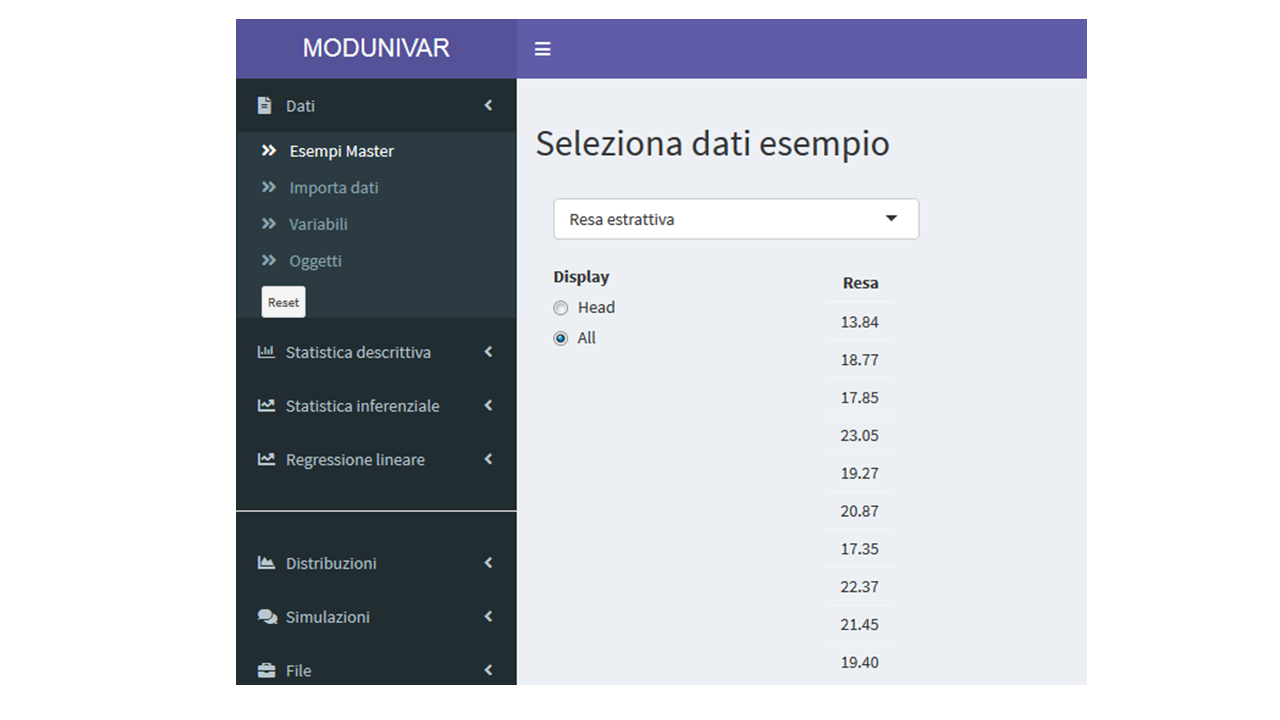
\includegraphics[width=1\linewidth]{Immagini/Descrittiva/1_Resa_estrattiva} 

}

\caption{Il dataset Resa estrattiva tra gli esempi didattici a disposizione per le lezioni del Master ECAIF}\label{fig:sd1}
\end{figure}

La prima funzione descrittiva che di solito si usa è quella di mettere i dati in una tabella: nel menu ``statistica descrittiva'' la voce ``Vedi dati'' consente di stampare in una tabella le misure.

\begin{figure}

{\centering 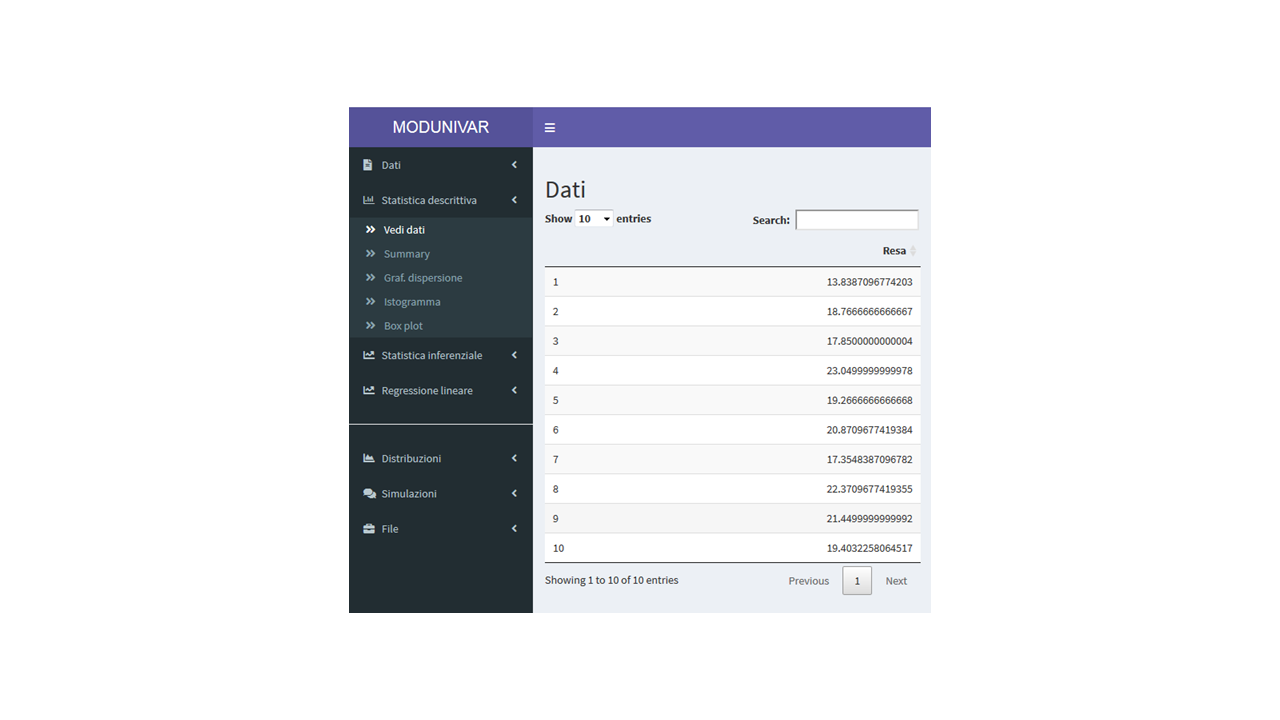
\includegraphics[width=1\linewidth]{Immagini/Descrittiva/2_TabelladatiResa estrattiva} 

}

\caption{Il dataset Resa estrattiva rappresentato in forma di tabella}\label{fig:sd2}
\end{figure}

L'informazione fornita da dieci numeri presentati in forma di elenco però può non essere molto utile, e pertanto spesso si preferisce presentare sia i valori grezzi in forma analitica sia i descrittori di posizione e dispersione dello stesso gruppo di dati. Selezionando la voce ``Summary'' dal menu ``Statistica descrittiva'', la funzione produce la stampa di media aritmetica (mean), deviazione standard (sd), intervallo interquartile (Inter-Quartile Range, IQR, differenza tra il terzo e il primo quartile, v. Glossario), valore minimo della serie (0\%), valore al primo quartile (25\%), mediana (50\%, secondo quartile), valore al terzo quartile (75\%), massimo (100\%) e numero di dati su cui si calcola la statistica.

\begin{figure}

{\centering 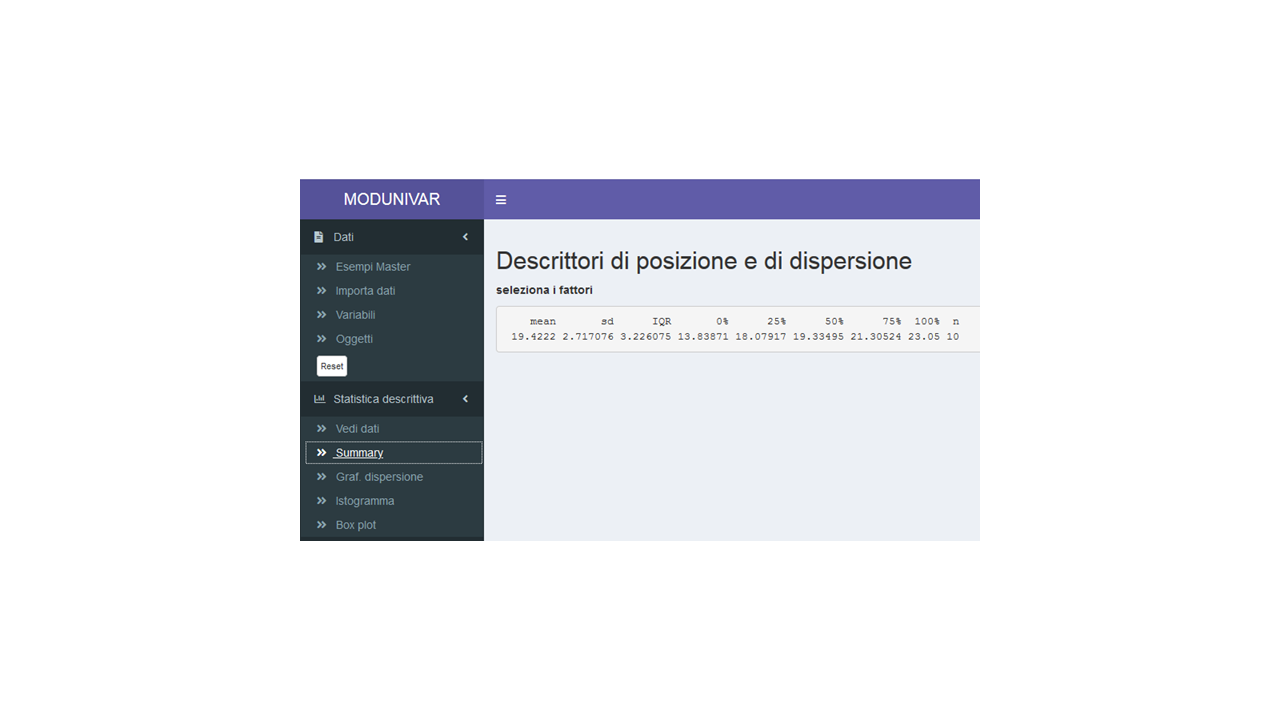
\includegraphics[width=1\linewidth]{Immagini/Descrittiva/3_SummaryResa_estrattiva} 

}

\caption{Indicatori di posizione e dispersione calcolabili dal dataset Resa estrattiva}\label{fig:sd3}
\end{figure}

Il primo strumento grafico di immediata comprensione si ottiene con il comando ``Graf. dispersione'' che stampa il grafico a punti cosiddetto ``a dispersione'', per visualizzare i dati così come sono.
Nel grafico, le rese estrattive si leggono sulle ordinate, mentre in ascissa compare il numero di ordinamento dei dati. La linea blu orizzontale indica il valore della media.

\begin{figure}

{\centering 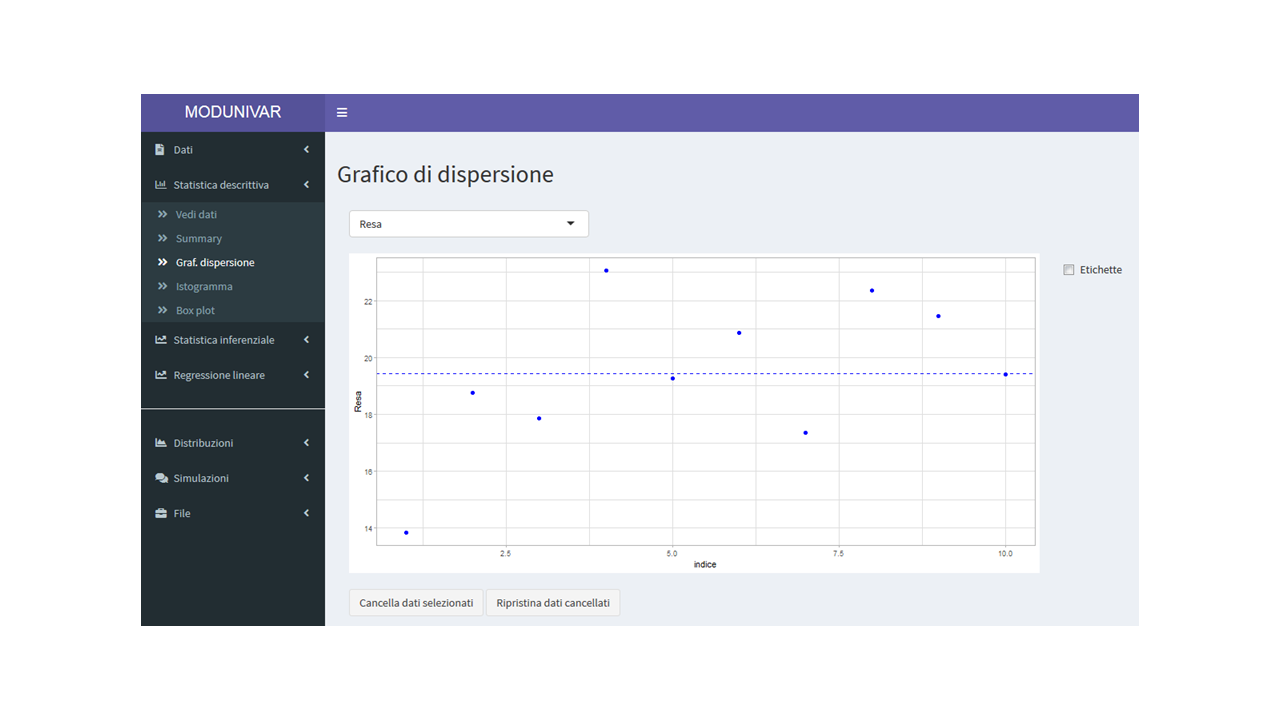
\includegraphics[width=1\linewidth]{Immagini/Descrittiva/4_Graf_dispers Resa_estrattiva} 

}

\caption{Grafico di dispersione dei dati di Resa estrattiva}\label{fig:sd4}
\end{figure}

Il grafico a punti può essere modificato introducendo le ``etichette dei dati'' che, in questo caso, coincidono con il numero di ordinamento dei dati.

Nelle relazioni con dati, è molto frequente incontrare grafici a barre, chiamati Istogrammi. Per ottenere una rappresentazione dei dati del dataset in forma di istogramma è sufficiente selezionare la voce ``Istogramma'' del menu ``Statistica descrittiva''. L'istogramma è un grafico in cui in ordinata sono riportate le rese raggruppate in intervalli definiti attrverso il comando ``larghezza barra''. In ordinata invece è possibile scegliere la forma dei dati da riportare tra tre possibilità: il conteggio dei dati che cadono negli intervalli di resa identificati attraverso il comando ``larghezza barra'', la percentuale del numero di questi dati sul totale dei dati raccolti (percentuale = 100·numero di dati che cadono nell'intervallo dato/10) e la loro densità (densità = area della barra = percentuale/100).

\begin{figure}

{\centering 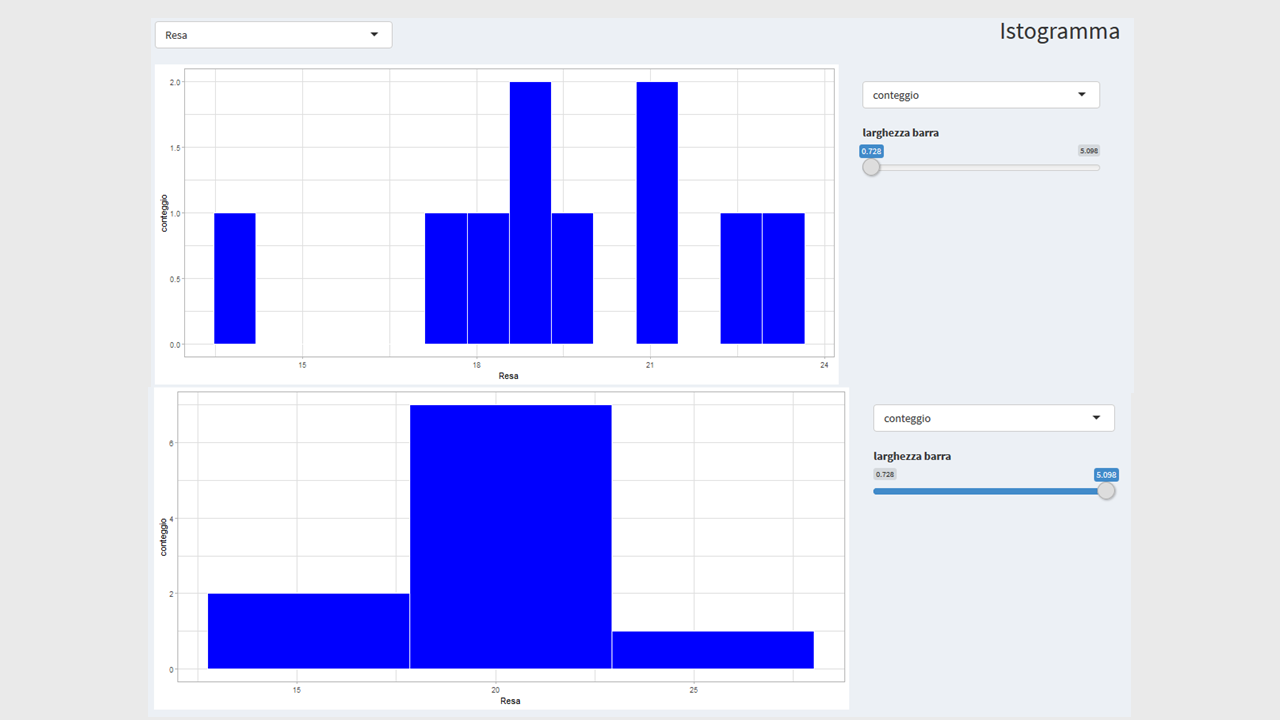
\includegraphics[width=1\linewidth]{Immagini/Descrittiva/5_IstogResaestrattiva} 

}

\caption{Istogrammi dei dati di Resa estrattiva. In alto, la larghezza delle barre è la minima possibile; in basso la larghezza delle barre è la massima possibile}\label{fig:sd5}
\end{figure}

Un altro importante strumento grafico è il ``box-and-whiskers plot'' (o boxplot), che si ottiene usando la funzione Box plot del menu ``Statistica descrittiva''. Il boxplot rappresenta in modo compatto in un unico grafico i maggiori descrittori dei dati.

\begin{figure}

{\centering 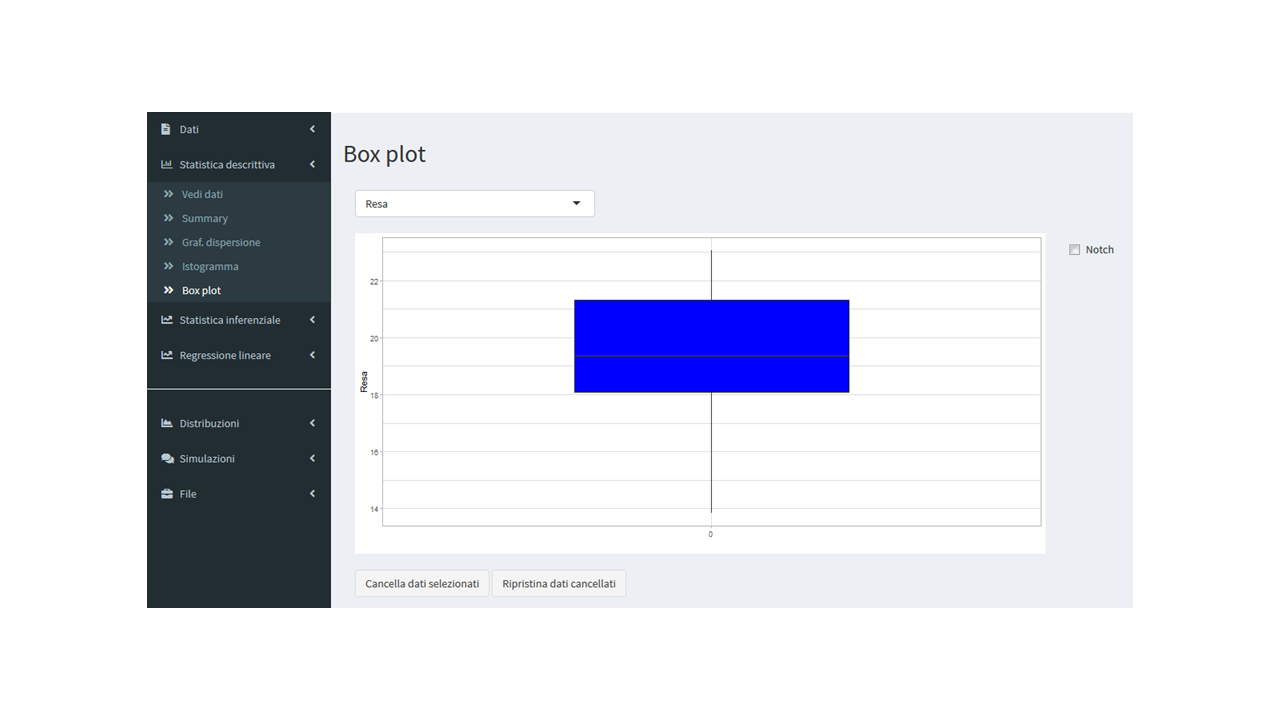
\includegraphics[width=1\linewidth]{Immagini/Descrittiva/6_BoxplotRestrattiva} 

}

\caption{Boxplot dei dati di Resa estrattiva}\label{fig:sd6}
\end{figure}

In ascissa compare un numero di ordine della serie di dati (in questo abbiamo una unica serie e viene assegnato di default il valore ``0'' in ascissa), mentre in ordinata sono riportati i valori di resa etrattiva. La ``scatola'' si estende dal primo al terzo quartile, la riga centrale rappresenta la mediana e i baffi vanno dal valore minimo al valore massimo. I baffi permettono anche di identificare valori anomali (dati aberranti, outliers). Una convenzione grafica accettata è che i dati che cadono fuori dalla scatola ad una distanza di almeno 1.5 volte la dimensione della scatola siano da considerare con sospetto e siano soggetti a verifica con opportuni test per gli outliers (test di Dixon, Grubbs, Cochran o altri).
Si osservi che il valore 1.5 è definito in automatico arbitrariamente dalla routine e nei software di statistica ``aperti'' può essere modificato.

\backmatter

  \bibliography{book.bib}

\addcontentsline{toc}{chapter}{Bibliografia}

\end{document}
